\documentclass{llncs}
\usepackage{graphics}
\usepackage[dvips]{epsfig}
\usepackage[latin1]{inputenc}
\usepackage{color}
\usepackage{longtable}
\usepackage{multirow}
\usepackage[dvips]{graphicx} 
%\usepackage{amsmath}
\usepackage{textcomp}
\usepackage{url}

\newcommand{\tab}{\hspace{20mm}}

\setlength{\textfloatsep}{8pt plus 2pt minus 2pt}
\setlength{\intextsep}{8pt plus 2pt minus 2pt}

%#\def\BibTeX{{\rm B\kern-.05em{\sc i\kern-.025em b}\kern-.08em
%#    T\kern-.1667em\lower.7ex\hbox{E}\kern-.125emX}}

%\hyphenation{}


\begin{document}

%%%%%%%%%%%%%%%%%%%%%%%%%%%%%%%   TITLE   %%%%%%%%%%%%%%%%%%%%%%%%%%%%%%%

\title{Evolving Galactic Conquerors}

%\thanks{\footnotesize{This work has been supported in part by project P07-TIC-03044, awarded by the Andalusian Regional Government.}}}

\titlerunning{Evolving Galactic Conquerors}

%%%%%%%%%%%%%%%%%%%%%%%%%%%%%%%   AUTHORS   %%%%%%%%%%%%%%%%%%%%%%%%%%%%%%%

%\author{A.F. Ares\inst{1} \and A.M. Mora\inst{1} \and P.A. Castillo\inst{1} \and J.J. Merelo\inst{1} \and M.G. Arenas\inst{1} \and R. Dugo\inst{1} ...}
%\authorrunning{A.F. Ares et al.}
%
%\institute{Departamento de Arquitectura y Tecnolog\'{\i}a de Computadores.\\
%Universidad de Granada (Spain)\\
%\email{\{antares,amorag,pedro,jmerelo,maribel\}@geneura.ugr.es}
%}

\maketitle

%
%%%%%%%%%%%%%%%%%%%%%%%%%%%%%%%   ABSTRACT   %%%%%%%%%%%%%%%%%%%%%%%%%%%%%%%
%
\begin{abstract}
In spite of the increase of interest in applying computational
intelligence techniques to computer games, there is one type that has
not received so much attention: real-time strategy (RTS) games, where traditional artificial intelligence techniques fail to play at a human level because of the vast search spaces that they entail.
We propose to make use of evolutionary algorithms fine-tune the
behavior of a bot that play Planet Wars, the game that has been used
for the Google Artificial Intelligence Challenge 2010.
The behavior engine of the proposed bot is based on a set of rules
established by means of exhaustive experimentation, followed by the
application of an evolutionary algorithm to determine the constants needed by those
rules. The resulting bot is able to beat the opponent (used to design it in the most challenging maps) and is well-placed (top 10\%) in the Google AI
challenge. 


\end{abstract}

%
%%%%%%%%%%%%%%%%%%%%%%%%%%%%%%%   INTRODUCTION   %%%%%%%%%%%%%%%%%%%%%%%%%%%%%%%
%
\section{Introduction and Problem Description}
\label{sec:intro}
%

A \textit{Bot} in a computer game environment usually designs as an
autonomous agent, which tries to compete in the game under the same
conditions as a human player and
cooperates with or fights/competes against a human player or other
bots. Bots have been used extensively in First Person Shooter (FPS)
games
\cite{laird2001using,ControllingBot_CEC2010,cooperativebots_CIG2010,Agent_Smith_CEC2009},
where the human players fight in an scenario (or arena) against some
of these bots, also known as Non-Playing Characters (NPCs). 

Real-time strategy (RTS) games are those where the player owns some
units (and/or structures) which he has to control, in order to beat
the opponent, usually in a battle. In a typical RTS it is possible to
create additional units and structures during the course of a
game. This is generally limited by a requirement to expend accumulated
resources. These are strategy-based games that usually work in real
time, without any player stopping to wait for the results of the moves
of the other player. Some examples of this type of game are the
famous Command and Conquer\texttrademark, Starcraft\texttrademark,
Warcraft\texttrademark~ or Age of Empires\texttrademark~ sagas.  

%A shortcoming of the AI used by bots in commercial games is that the methods employed (such as finite state machines, expert systems and rule-based systems) are hard-coded, and hence are static and require hand-tuning of parameters \cite{falke2003,ontanon2007}. 

%In the recent years, the application of computational intelligence methods have arisen, in order to improve an existing decision engine. This is done by changing the parameters on which it depends, or by means of the design of the whole set of rules which models the behavior.

RTS games are inherently difficult for its real-time nature (which is
usually addressed by constraining the time that must be used to reach
a decision) and also for the huge search space that is implicit in its
action. This is probably one of the reasons why in the last
Computational Intelligence in Games conference (IEEE-CIG 2010), just a
few papers deal with this kind of games; the table of contents reveals
just three papers, out of sixty, dealing with the subject. That is
probably also one of the reasons why Google has chosen this kind of
game for their Artificial Intelligence Challenge 2010.

The objective of the work presented in this paper is to implement the
decision engine for a bot that plays a RTS game called
\textit{Planet Wars} or Galcon \cite{wiki:galcon}, which has been chosen for the Google AI
Challenge 2010 \cite{webGAIC}. This decision engine has been designed
in two steps: first, a set of rules has been defined by means of
exhaustive experimentation; they model the behavior of the bot, and depend on some parameters. 
The second step has been the application of a Genetic Algorithm (GA) \cite{GAs_Michalewicz96} 
to evolve (and improve) these parameters off-line (not during a match, but previously to the game fights). 

The rest of the paper is structured as follows: 
Section \ref{sec:planet_wars} describes the problem by presenting the Planet Wars game. 
Section \ref{sec:stateofart} reviews related approaches to behavioral engine design in similar game-based problems.
Section \ref{sec:genebot} presents the proposed method, termed {GeneBot}, detailing the finite state machine and the parameters which model its behavior, in addition to the GA which evolves them.
The experiments and obtained results are described and analyzed in Section \ref{sec:experiments}.
Finally, the conclusions and future lines work are presented in Section \ref{sec:conclusions}.

%%%%%%%%%%%%%%%%%%%%%%%%%%%%% PROBLEM DESCRIPTION %%%%%%%%%%%%%%%%%%%%%%%%%%%%%
\section{The Planet Wars Game}
\label{sec:planet_wars}

The Planet Wars game chosen for the Google AI challenge (GAIC) \cite{webGAIC}
is an artificial intelligence competition where game-playing programs
fight against others programs. As previously stated, our aim is to
design the behavioral engine of a bot that play Planet Wars as well as possible. So it
will try to win against any enemy (usually other bots). 

Planet Wars is a game based on Galcon \cite{wiki:galcon}, but is designed to be simpler, since it is addressed to held bot's fights. The contest version of the game is for two players.

\begin{figure}[ht]
\begin{center}
  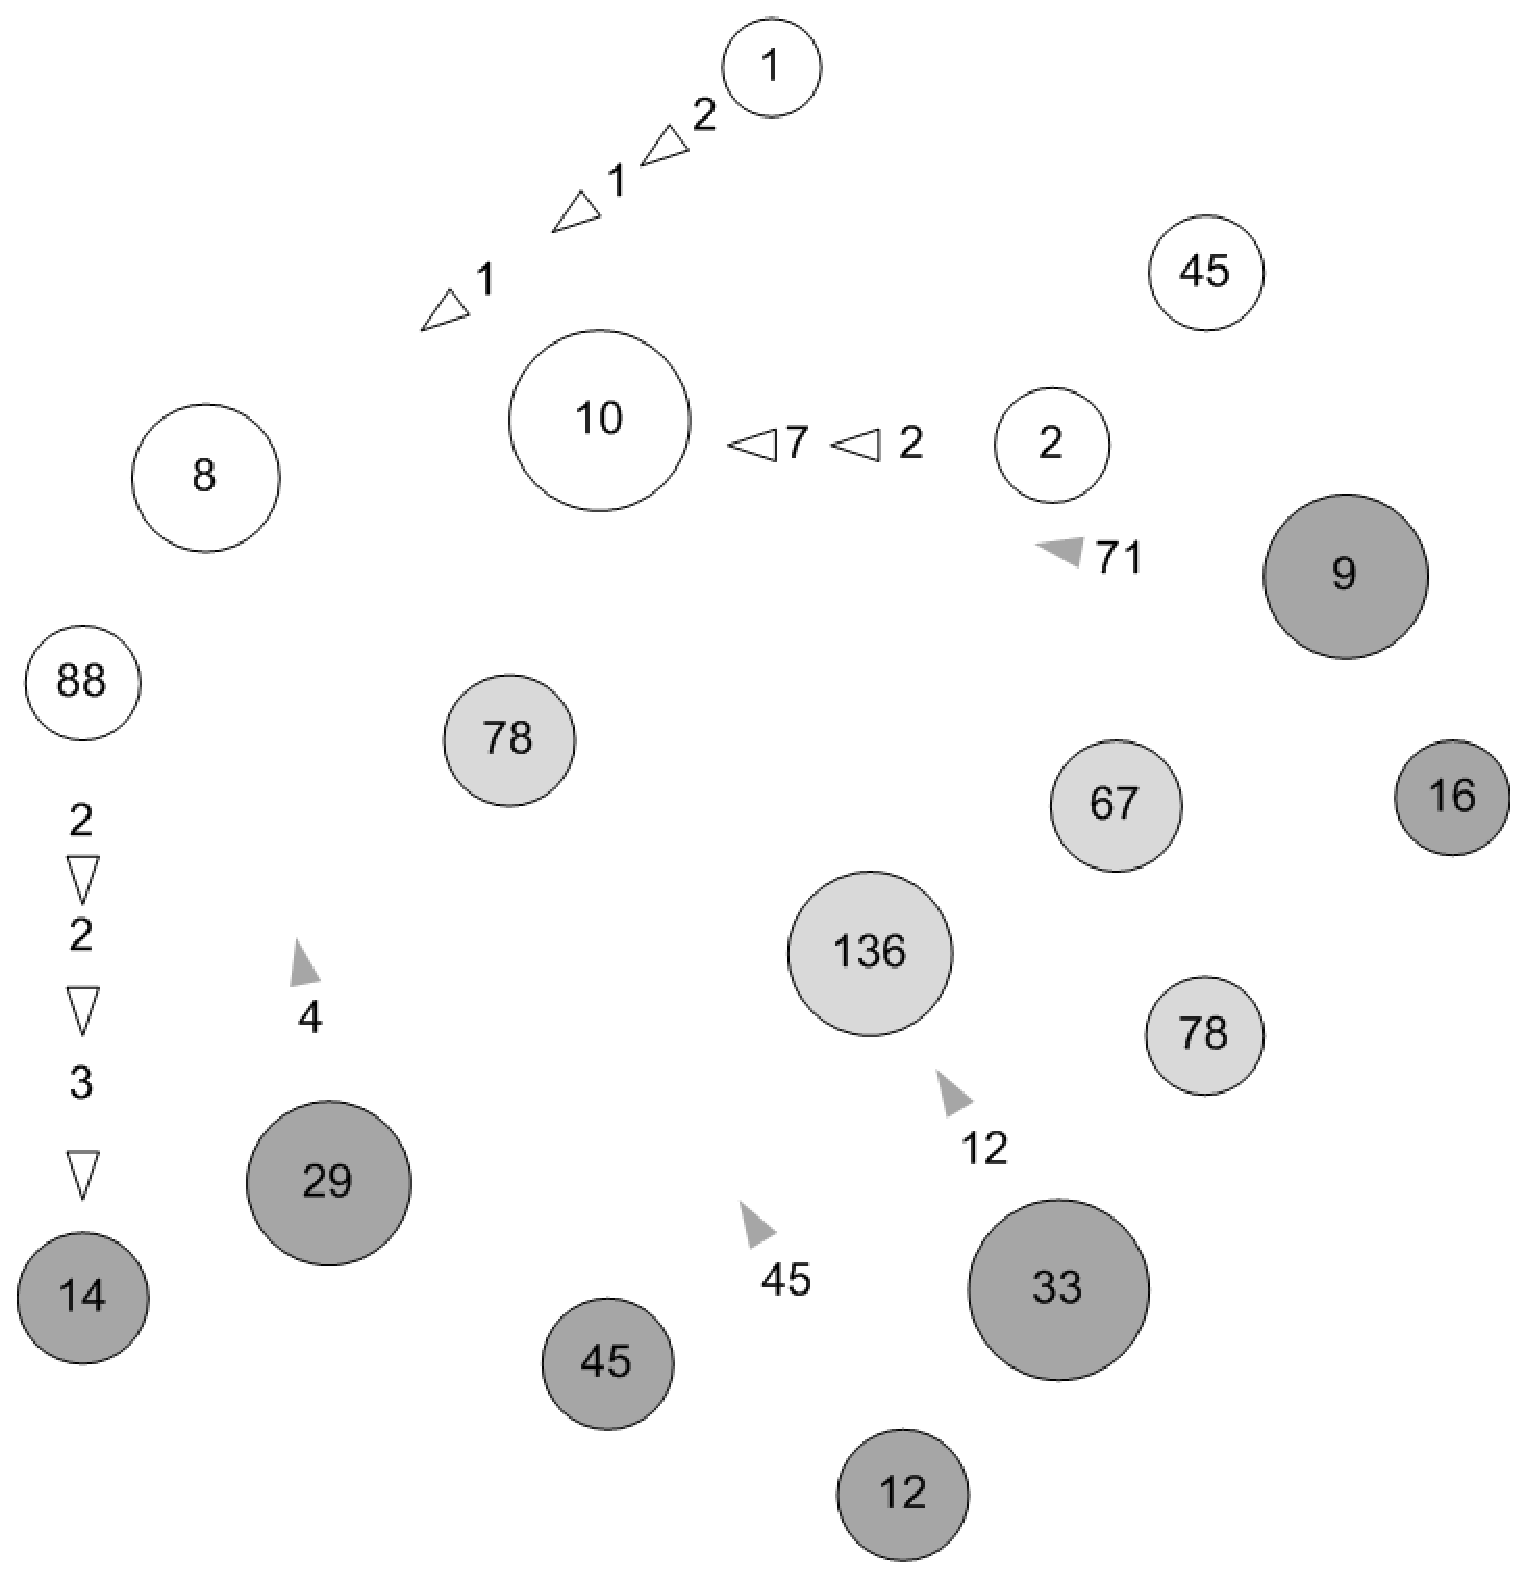
\epsfig{file=./imagenes/naves.eps,width=5cm}
\end{center}
\caption{Simulated screenshot of an early stage of a run in Planet Wars. White planets belongs to the player (blue color in the game), dark grey are planets are enemy's (red in the game), and light grey planets are nobody's. The triangles are fleets, and the numbers (in planets and triangles) mean starships.}
\label{figura:PlanetWars1}
\end{figure}

A Planet Wars match takes place on a map which contains several
planets, each of them with a number on it that represents the number
of starships it hosts (see Figure \ref{figura:PlanetWars1}). Each
planet may have a different number of starships, and may belong to one
of three different owners: the player, the enemy, or neutral
(nobody). Ownership is shown with a colour, being blue for the
player, red for the enemy, and grey for neutral (a non-playing character). 

The objective is to defeat all of your opponent's planets. Even if it
is a real-time game, the implementation is turn-based, with is a
maximum number of turns to accomplish this objective. The player with
more starships at the end of the match (set to two hundred turns in
the challenge) wins, but if both players have
the same number of forces when the game ends, it is a draw. 

Each \textbf{planet} has some properties: \textit{X and Y
  Coordinates}, \textit{Owner's PlayerID}, \textit{Number of
  Starships} and \textit{Growth Rate} (on which depend the increasing
of the number of starships in it). Players send fleets to conquer
other planets (or to reinforce its own), and every \textbf{fleet} has
the properties: 
\textit{Owner's PlayerID}, \textit{Number of Starships},
\textit{Source PlanetID}, \textit{Destination PlanetID}, \textit{Total
  Trip Length}, and \textit{Number of turns remaining until arrival}. 

Each autonomous bot is implemented as a function that takes a list of
planets and  fleets, each one with the properties shown above, and
outputs orders as a text file; in each turn, the player has to choose
where to send fleets of starships, departing from any of his planets,
to any other planet on the map. The fleets can take some turns to
reach their destination. When a fleet reaches a planet, then it fights
against the existent enemy's forces (losing one starship for each one
at the planet) and, if it outnumbers the enemy units at the planet
he/she becomes owner of that planet. If the
planet already belongs to him, the incoming fleet is added as
reinforcement. Each planet owned by a player (but not the ``neutral''
ones) will increase
the forces there according to that planet's growth rate.  

So, the problem to solve is the design of the function that considers
the state of the map in each turn and decides the actions to perform
in order to get and advantage over the enemy, and at the end, win the
game.

There are two important constraints in the Google AI
challenge: the first one is that a bot cannot keep any data from one
turn to another (there is no memory). The second one is that the time
limit to (decide and) perform the actions is just one second.

These restrictions make it difficult to implement an on-line
metaheuristic approach, so our we run the evolutionary algorithm
off-line and one a satisfactory state is found, it is sent to fight at
the Challenge. Next we will see how other strategies for games have
been designed. 


%%%%%%%%%%%%%%%%%%%%%%%%%%%%%%  STATE OF THE ART  %%%%%%%%%%%%%%%%%%%%%%%%%%%%%
%
\section{State of the Art}
\label{sec:stateofart}
%

In relation with the design or improvement of the Bots' AI in computer games,
most attention has been directed at in FPS, starting
with Doom\texttrademark~ or
Quake\texttrademark~\cite{laird2001using} by the beginning of the 90s;
more recently, the most important game (or environment) in which these
studies have been developed is Unreal
Tournament\texttrademark~\cite{Agent_Smith_CEC2009,ControllingBot_CEC2010,cooperativebots_CIG2010}.  

The behavior in these bots has been designed following different
approaches: parameter-tuning based methods using reinforcement learning
\cite{mcpargalCIG2008} of genetic algorithms to
tune up the parameters of an expert system that controls the
bots \cite{colomiCEC2004}. More complex approaches involve artificial
Neural Networks (NNs) trained with reinforcement learning
\cite{NN_FPS_IEICE2006}, or neural nets evolved for optimizing several
objectives at the same time\cite{schrummiikkuCIG09}. 
Some recent papers, such as \cite{ControllingBot_CEC2010}, use both approaches
described above at the same time: a genetic algorithm evolves the
parameters of the Fuzzy Finite State Machine (FFSM) included in the
game core that controls the bot's behavior, and a genetic programming
to evolve rules as a replacement for the FFSM ones.  

There are not so many papers devoted to RTS games, such as Age of
Empires\texttrademark~ or Starcraft\texttrademark;
\cite{hongchoCIG2005} is an example. However, in many RTS games,
traditional artificial intelligence techniques fail to play at a human
level because of the vast search spaces that they entail. In this
sense, Ontano et at. \cite{ontanon2007} proposed to extract
behavioral knowledge from expert demonstrations in form of individual
cases. This knowledge could be reused via a case based behavior
generator that proposed advanced behaviors to achieve specific
goals. Other authors propose using coevolution for evolving team tactics
\cite{avery2010coevolving}. However, the problem is how tactics are
constrained and parametrized and how is the overall score computed. 

On the other hand, RTS games usually have a 'static' or scripted (it
does not change nor evolve) AI that controls the computer's
actions. Once the user has learnt how such a game will react, the game
quickly loses its appeal. In order to improve the users' gaming
experience, Falke et al. \cite{falke2003} proposes a learning
classifier system that can be used to equip the computer with
dynamically-changing strategies that respond to the user's strategies,
thus greatly extending the games playability. 

%%%  Something about Google AI Challenge in previous years (if it was performed).

Applying evolutionary algorithms to a parametrized tactic is
relatively novel, and, as far as we know, nobody has applied it to
this game, although the game forum mentions another challenger using
genetic programming to evolve tactics. The idea in this work is to
apply an evolutionary approach (mixed with 
some behavior model rules) to built the decision engine of a bot for
playing in a 'simple' RTS game, getting advance of the best of both
techniques. 
% Antonio - no se si ha quedado bien, echadle un ojillo a ver. ;):D


%%%%%%%%%%%%%%%%%%%%%%%%%%%%%%%%  GENETIC BOT  %%%%%%%%%%%%%%%%%%%%%%%%%%%%%%%%
%
\section{GeneBot: The Galactic Conqueror}
\label{sec:genebot}
%

As previously stated in Section \ref{sec:planet_wars}, the main
constraint in each turn is the little processing time
available to perform the correspondent actions (1 second). In
addition, there is another key constraint, the complete
absence of memory from one turn to another. These restrictions have
strongly limited the design and implementation possibilities for our
bot, since almost all the metaheuristics are based in a memory of
solutions or the assignment of payoffs to previous actions in order to
improve future behavior, and most of them are quite expensive in
running time; running an evolutionary algorithm each turn, for
instance, or a Monte Carlo method is almost impossible. Besides, just
the overall result of the strategy can be evaluated, 
without being able to optimize individual actions due to the lack of
feedback from one turn to the next. 
% Antonio - estas afirmaciones son un poco vagas...

These are the reasons why we have decided to define a set of rules
which models the on-line (during the game) bot's AI. These rules have
been formulated through exhaustive experimentation, and strongly
depend on some key parameter, which determines in the end the
behavior of the bot. 
%These parameters are composed by the game information in each turn.
% Antonio - esto no se si es del todo cierto... 
% Yo creo que no, por eso lo he cambiado.
These parameters will be computed offline using an evolutionary
algorithm, and fixed when the bot is sent off to fight to distant
planets with other Google AI challengers. The number and nature of
these parameters will be explained below. 

This way, the main idea is to perform an off-line parameter
optimization, by applying a Genetic Algorithm (GA)
\cite{GAs_Michalewicz96}, so the resulting bot has been
designed \textit{GeneBot}. In this optimization step, our bot
fights against a standard Google bot, which is included in the game
kit that can be downloaded from the GAIC site, is quite
simple but works very well in most of the game maps. It works as
follows: for a state of
the map, it seeks the planet that hosts most ships and the best planet
to attack by calculating the ratio between the growth-rate and the
number of ships. It attacks a single planet at a time, toggling
between attack and non-attack modes; this one taken when it is under
attack. Despite its simplicity it manages to win in enough maps if his
opponent is not good enough.  %(in fact, it defeats GAIBOT in a map). % Contra quién? - JJ %Antares - Vale, está mal
      % precisado. Me refiero a que es capaz de ganar en todos los tipos
      % de mapas (de hecho al GAIBOT le gana en uno de los mapas). De
      % hecho, las primeras versiones del bot perdían contra él muchas
      % veces. E icluso, muchos de los individuos generados en el
      % genético no conseguían ganarle. 
In fact the Google AI Contest recommends that any
candidate bot should be able to always win the standard Google bot in
order to have some kind of chance in the hall of fame; this is the
baseline for even considering the bot as a challenger, and the number
of turns it needs to win is an indicator of its quality. 

From this standard bot, we derive another, which we call GAIBOT (Google
AI Bot) whose strategy derives from this one, but with small
variations. This bot works as follows: At the beginning of a turn, the bot tries to find a \textit{base
  planet}, decided on the basis of a score whose weights will be evolved. The rest of the planets are named \textit{colonies}.
Then, it determines which \textit{target planet} to attack (or to reinforce) in 
the next turns (since it can take some turns to get to that planet). 
If the planet to attack is neutral, the action is termed \textit{expansion}; 
however, if the planet is owned by the enemy, the action is named 
\textit{conquest}. The internal flow of the behavior of GeneBot with
these states is shown in Figure
\ref{figura:diagram}. 
%
\begin{figure}[ht]
\begin{center}
  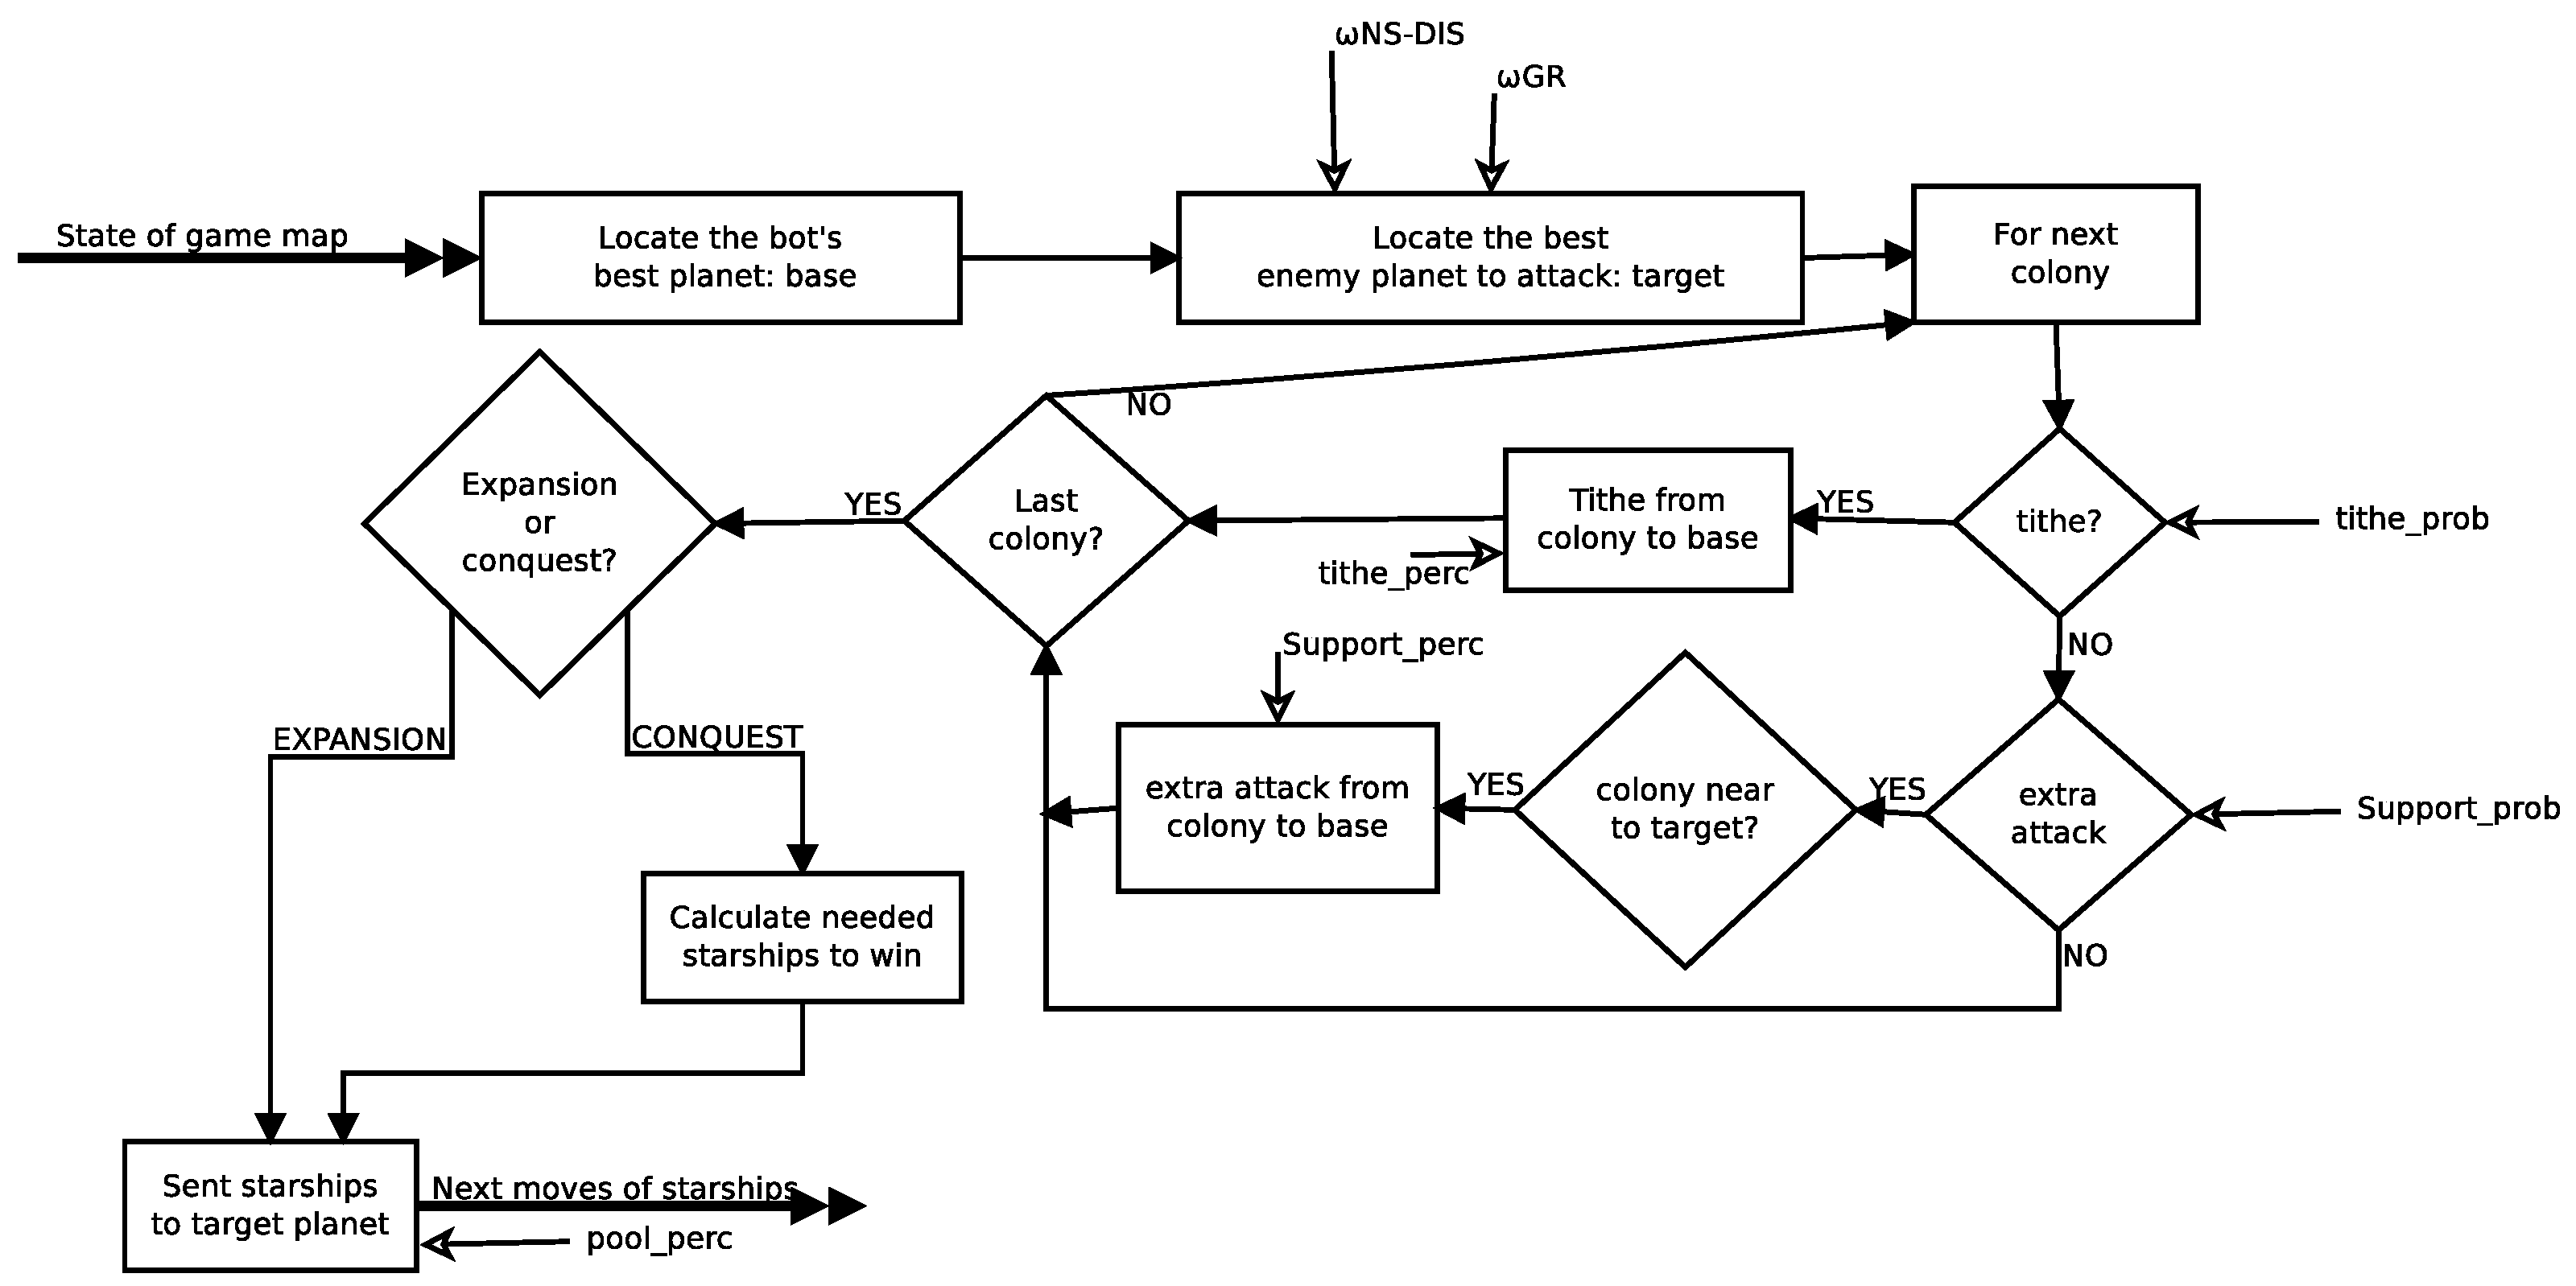
\epsfig{file=imagenes/Diagrama1.eps,width=12cm}
\end{center}
\caption{GeneBot behavior finite state machine. It is shown where is considered each one of the parameters to evolve.}
\label{figura:diagram}
\end{figure}
%

The function considered to select the \textit{target planet} is as follows:

\begin{footnotesize}
\begin{equation} \label{eq:fitness_ga}
Score(p)= \frac {p.NumStarships \cdot \omega_{NS-DIS}\cdot Dist(base,p) } {1 + p.GrowthRate \cdot 
\omega_{GR} }
\end{equation}
\end{footnotesize}

\noindent where $\omega_{NS-DIS}$ and, $\omega_{GR}$ are weights related to the number of starships, the growth rate and the distance to the target planet. These values are adjusted using the GA, and will be commented in the next section. 
$base$ is the best planet of the bot, and $p$ is the planet to evaluate. The addition of '1' in the divisor ensures not to perform a division by zero.

Once the target enemy planet is designed, a particular colony can
provide a part of its starships to the base planet.
Moreover, if the distance between the colony and the target planet is less than the distance between the base and target planet, there is a likelihood that the colony also sent a number of troops to the target planet. 
%Tithing and the attack of colonies are disjoint, both can not happen in the same turn for a particular colony.

%Una vez programados los envíos de las tropas de diezmo y ataque desde las colonias, se envía el resto de tropas desde el planeta base. En caso de que estemos expandiendo, el planeta no tendrá generación de tropas por lo que se mandarán las tropas necesarias para conquistar el planeta más un número determinado de naves extras. En caso de que se esté conquistando, el envío de tropas tendrá en cuenta la generación de tropas del planeta objetivo mientras las tropas llegan hasta su objetivo.

Once tithe and attack fleets from the colonies are scheduled, the remaining starships from the planet base are sent. 
If it is in expansion, the planet will not generate starships, so
enough effectives to conquer the target planet will be sent with a
certain number of extra units; this number is adjusted using the GA, and will be also commented in the next section. 
If it is trying to conquer a planet, the bot estimates the number of starships (grouped in fleets) needed to do it.

The following sections present the parameters which have been optimized
using the GA, and the implemented algorithm to perform the optimization
process. GAIBOT has intuitive and hand-fixed values for all weights
mentioned; they are shown in Table \ref{tab:tabla_valores}. However, to evolve
galactic conquerors we will leave all parameters as variables that will
have to be optimized by the evolutionary algorithm. These parameters
will be explained in the next section. 

%------------------------------------------------------

\subsection{Parameters to Optimize}
\label{subsec:parameters}

The set of parameters is composed by some weights, probabilities and amounts, that have been included in the rules that model the bot behavior (see them in the diagram in Figure \ref{figura:diagram}). They have been determined following a systematic experimentation method, and have a strong influence in determining the final behavior of the bot:

\begin{itemize}

%%%
%	\item \textbf{diezmo}: Es el número de tropas que son enviadas (en porcentaje a las tropas almacenadas en el planeta) que serán enviadas en el diezmo. [0,1]
%	\item \textbf{p\_diezmo}: Es la posibilidad de que una colonia envie un diezmo a la base. [0,1
%	\item \textbf{p\_NS}: Es el peso del número de planetas que almacena el planeta en la función de selección del planeta objetivo. [0,1
%	\item \textbf{p\_GR}: Es el peso del factor de crecimiento del planeta en la función de selección del planeta objetivo. [0,1]
%	\item \textbf{p\_DIS}: Es el peso de la distancia en la función de selección del planeta objetivo [0,1]
%	\item \textbf{flotas\_extras}: Es el número de flotas extras enviadas en los ataques a los planetas. [0,1]
%	\item \textbf{envio\_secundo}: Es el número de flotas enviadas (en porcentaje a las tropas almacenadas en el planeta) que serán enviadas en el envío de tropas auxiliar. [0,1]
%	\item \textbf{p\_envio\_segundo}: Es la posibilidad de que una colonia envíe tropas al planeta objetivo [0,1]
%%%
	\item $tithe_{perc}$:  percentage of starships the bot sends (regarding the number of starships in the planet).

	\item $tithe_{prob}$: probability that a colony sends a tithe to the base planet.

	\item $\omega_{NS-DIS}$: weight of the number of starships
          hosted at the planet and the distance from the base planet
          to the target planet; it is used in the score function of
          target planet. 

	\item $\omega_{GR}$: weight of the planet growth rate in the target planet score function.

	\item $pool_{perc}$: proportion of extra starships that the bot sends from the base planet to the target planet.
	
	\item $support_{perc}$: percentage of extra starships that the bot sends from the colonies to the target planet.

	\item $support_{prob}$: probability of sending extra fleets from the colonies to the target planet.

\end{itemize}

Each parameter takes values in a different range, depending on its meaning, magnitude and significance in the game, but all of them are normalized to the $[0,1]$ range.

%That range has been established, conforming a width interval when the parameters are just modifiers (they are added or subtracted), and a short one if they are considered as one of the main factors in the bot's decision taking, to avoid an extremely bad behavior.
% Antonio - esto no se si es cierto, pero debería. XD

The problem is to find the best parameter values in order to get the most suitable bot's behavior. Even finding the relative importance of each of them in the bot' AI modeling.
To do this, a GA has been applied, as is commented in the next section.

%------------------------------------------------------

\subsection{The Genetic Algorithm}
\label{subsec:theGA}

The implemented GA follows a \textit{generational}
\cite{GAs_Michalewicz96} scheme, considering \textit{elitism} to
maintain the best solutions in time. Each individual (chromosome) is a
floating point number array, with each component corresponding to one of parameters (see \ref{subsec:parameters}). 

The genetic operators include a \textit{BLX-alpha} crossover
\cite{Herrera03ataxonomy} (with alpha equal to 0.5) and a \textit{gene
  mutator} which mutates the value of a random gene by adding or
subtracting a random quantity in the $[0,1]$ interval. 
% ¿Qué pasa si el resultado excede el máximo o mínimo del intervalo? - JJ - Antares - El blx-alfa controla que no se superen esos umbrales y la mutación genera un número entre esos valores, por lo que no hay problemas.

%Each operator have an application rate (0.6 for crossover and 0.02 for mutator).

%Regarding the GA genetic operators \cite{EvoCompI,Michalewicz2004}, a \textit{BLX-alfa crossover} \cite{Herrera03ataxonomy} and a \textit{simple gene mutation} (change the value of a random gene -or none- by adding or subtracting a random quantity in [0,1]). 
The \textit{selection mechanism} implements a \textit{2-tournament}
\cite{EvoCompI}. % Por qué ese número? Se han probado otros? - JJ - Antares: Vaya, no había cazado ese error. El torneo se hizo al final contra dos individuos, ya que con 6 los peores individuos tenían menos posibilidad de reproducirse. Si, se probaron varios valores, el nombrado 6, 4 y finalmente 2, que fue lo que se consideró más correcto según el tamaño de la población que manejabamos. En un correo Juanlu me recomendaba, que para el tamaño de población que teníamos, 2 era un valor bastante bueno. 
The elitism has been implemented by replacing a random individual in
the next population with the global best at the moment. The worst is
not replaced in order to preserve diversity in the population.
% Esto es peligroso; si el peor no se reproduce en la siguiente
% generación no contribuye absolutamente nada. En ese sentido, es
% mejor reemplazar a los peores que a otro cualquiera, porque, total,
% no van a servir pa ná. Por favor, aclarar eso o poner otra
% justificación. - JJ
% Antares - Lo que hice fue, una vez que se generaban los nuevos individuos de una generación x+1, su cuatro peores individuos eran remplazados por los 4 mejores individuos de la generación X. No sé si esto estará bien hecho o no...

The evaluation of one individual is performed by setting the correspondent values in the chromosome as the parameters for GeneBot's AI, and placing the bot inside a scenario to fight against a GAIBOT. 
% This bot is fighting for 5 matches, once they have finished, the individual 
% % Antonio - El bot combate en 5 escenarios diferentes, ¿no?
% % Antares - Así es, el bot se enfrenta en 5 escenarios diferentes y representativos de un tipo de mapa distinto.
% (chromosome which contains the parameters and models one behavior) is evaluated considering the fitness function:

% \noindent \ \ \ {\tt if(indiv1.wins != indiv2.wins)\{ }

% \noindent \ \ \ \ \ \ \ \ \ \ \ {\tt if(indiv1.wins == false) return 1 }

% \noindent \ \ \ \ \ \ \ \ \ \ \ {\tt if(indiv2.wins == false) return -1 }

% \noindent \ \ \ {\tt \} else \{ }

% \noindent \ \ \ \ \ \ \ \ \ \ \ {\tt if(indiv1.turns<indiv2.turns) return -1 }

% \noindent \ \ \ \ \ \ \ \ \ \ \ {\tt else if(indiv1.turns>indiv2.turns) return 1 }

% \noindent \ \ \ \ \ \ \ \ \ \ \ {\tt else return 0 }

% \noindent \ \ \ {\tt \} }

% \noindent \ \ \ {\tt return 0 }

% \noindent where \emph{indiv1.win} means that GeneBot has won, while \emph{indiv1.turns} stands for the number of turns GeneBot has played.
% Antonio - ¿qué son los dos individuos?¿no se evalúa solo uno?¿o se refiere al GAIBOT?
% Antares - Lo que se compara es la función de fitness de dos bots concretos. Esta función es utilizada en el torneo entre individuos a la hora de realizar un cruce.

% Maribel La primera frase creo que no es necesaria,

%La funci�n de fitness ejecuta el bot configurado (con los par�metros que indiquen los genes del indiviuo ) en el entorno del juego, en cinco mapas que han sido seleccionados por ser los m�s significativos (mapas con m�s planetas, menos planetas, el planeta que el bot sin mejorar no es capaz de ganar, el mapa que menos tarda en ganar y el mapa que m�s tarda en ganar). De dichas ejecuciones del bot en el entorno de juego, se calculan dos valores. El n�mero de turnos que ha tardado en ganar cada mapa y si ha perdido alguno de los mapas.

During the five matches, two values are calculated for the fitness
evaluation: the first one is the number of turns that the bot has
needed to win in each arena ($WT$), and the second is the number of
games that the bot has lost ($LT$). Every generation bots are ranked
considering the $LT$ value; in case of coincidence, then the $WT$
value is also considered as shown above: the best bot is the one that
has won every single game; if two bots have the same $WT$ value, the
best is the one that needs less turns to win.  This would probably be
done better in an multiobjective way, to give the evolutionary
algorithm a better chance of exploring the space; however, it is quite
clear that the most important thing is to win the most games, or all
in fact, and then minimize the number of turns; this way of ranking
the population can be seen as an strategy of implementing a
constrained optimization problem: minimize the number of turns needed
to win {\em provided that} the individual is able to win every single
game. 
% Antonio - este párrafo no se entiende bien y es reiterativo... primero se usa WT, si no, se usa LT (le he cambiado el nombre XD) y si es igual se usa WT...
Finally, in case of a complete draw (same value for LT and WT), zero is returned, meaning that no one has won.

% Maribel esto es un poco raro, por una parte se calculan el n\'umero de turnos que gana (en cada partida o en las cinco juntas) y el n\'umero de juegos que pierde ( pero ya de las cinco no? ) osea que por una parte el fitness tiene un valor de cada partida y otro valor de las cinco partidas?

% Maribel Creo que no me he enterado como se ordenan que alguien aclare como se ordenan los individuos porque la segunda parte no la entiendo.


%La funci�n de fitness del indiviuo ser� mejor cuanto menos turnos haya tardado en ganar siempre y cuando no haya perdido ninguna contienda. Si ha perdido alguna contienda, ser� peor que cualquier individuo que haya tardado m�s turnos siempre y cuando este haya ganado. En breve, se puede resumir as�:

  
%This function tries to promote \textbf{TO-DO: blablabla, because... (lo que me comento Antonio en uno de sus correos)... luego lo pongo}

% Antonio - ¿Se van a hacer bot especialistas o un bot genérico?
% Antares - Hubiese estado bien implementar lo del bot especialista, sin embargo, (además del tiempo) no fui capaz de encontrar una forma inmediata que indicase al bot en que tipo de mapa estaba.
% Antonio - ¿No hay búsqueda local? Siempre suelen decir que la metas... ;)

%%%%%%%%%%%%%%%%%%%%%%%%%%%%%%%   EXPERIMENTS  %%%%%%%%%%%%%%%%%%%%%%%%%%%%%%%%
%
\section{Experiments and Results}
\label{sec:experiments}
%
% Antonio - Comentar varias cosas
% - descripción de los mapas
% - número de experimentos en total
% - IA del bot Standard (aquí o antes cuando lo comentamos por primera vez)
% - forma y utilidades para hacer los experimentos (programas, forma de funcionamiento de cada experimento)
% - valores que se van a mostrar en las tablas
% ... más cosicas ...

To test the algorithm, different games have been played by pitting the
standard bot (GAIBOT) against the optimized bot (GeneBot). The
parameters considered in the GA are a population of 200 individuals,
with a crossover probability of 0.8 (in a random point) and a mutation
rate of 0.02. A two-individuals elitism has been implemented.  
%In the Table the experimental setup can be found
% Estos valores deberían justificarse - JJ
% Antares - ¿Cómo lo justificamos? :S El tamaño de población es lo suficientemente grande como para generar diversidad pero lo suficientemente pequeño como para que evaluar una generación no sea excesivamente costoso computacionalmente. La probabilida de cruce es alta, porque ya que implementamos elitimos no tenemos que controlar respecto con ella la permanencia de los mejores. Y el factor de mutación, del 2% es bastante arquetípico...
%\begin{table}[htp]
%\centering
%\begin{tabular}{|l|c|}
%\hline
%\textit{Number of individuals} & 400\\
%\textit{Mutation probability} & 0.02 \\
%\textit{Crossing probability} &  0.6 \\
%\hline
%\end{tabular}
%\caption{Parameters of GA.
%\label{tab:ga-params} }
%\end{table}

To evolve the behavior parameters, 30 runs of the GA have been performed, using 5 different (and representative) maps.

The evolutionary algorithm yields the values shown in Table \ref{tab:tabla_valores}. 

\begin{table}[htp]
\centering
\begin{tabular}{|l|l|l|l|l|l|l|l|l|}
\hline
           & $tithe_{perc}$ & $tithe_{prob}$ & $\omega_{NS-DIS}$ & $\omega_{GR}$ & $pool_{perc}$  & $support_{perc}$ & $support_{prob}$ \\
\hline
GAIBOT &        0,1 &        0,5 &          1 &          1 &          0,25 &        0,5 &        0,9 \\
\hline
GeneBot &      0,294 &     0,0389 &      0,316 &      0,844 &        0,727 &      0,822 &      0,579 \\
\hline 
\end{tabular}
\\[1ex]
\caption{Initial behavior parameters values of the original bot
  (GAIBOT), and the optimized values (evolved by a GA) for the best
  bot obtained using the evolutionary algorithm (GeneBot).
% Pero ¿GAIBOT usa exactamente las mismas fórmulas gue Genebot? Por
% cierto, no me gustan nada todo-mayúsculas, me gustaría más GeneBot -
% JJ 
% Antares - GaiBot usa las mismas reglas que el GeneBot, sin embargo, las fórmulas son distintas en cuanto los pesos, probabilidades y porcentajes son distintos. Consideramos que GaiBot es el bot antes de optimizar sus parámetros.
\label{tab:tabla_valores} }
\end{table}

Results in Table \ref{tab:tabla_valores} show that the best results
are obtained by strategies where colonies have a low probability of
sending tithe to the base planet (only 0.3), and those tithes send a
few hosted starships, which probably implies that colonies should be
left on its own to defend themselves instead of supplying the base
planet. On the other hand, the probability for a planet to send
starships to attack another planet is quite high (0.58), and the
proportion of units sent is also elevated, showing that it is more
important to attack with all the available starships than wait for
reinforcements. Related to this property is the fact that, when
attacking a target planet, the base one also sends a large number of
extra starships (72.7 \% of the hosted ships). Finally, to define the
target planet to attack, the number of starships hosted in the planet
is not as important as the growth range, but being the distance also
an important value to take into account.  
% Pero ¿se tiene en cuenta que las naves que se envíen sean más que
% las que hay? Porque si no se está haciendo de una torta un pan :-) -
% JJ 
% Antares - Obviamente, no va a intentar mandar más naves de las que él mismo tiempo. Todo este tipo de reglas está "implicitas" en la implementación. De hecho, intentar mandar más naves de las que un planeta tiene causa que el jugador que lo haya intentado pierda la partida.

After this experiments, the value of the obtained parameters has been
tested considering 100 different games (matches), where the 'evolved'
GeneBot has fought against a standard GAIBOT. The results are shown in
Table \ref{tab:resultados_tabla_resumen}. 

%\textbf{FERGUIMPORTANTE! lo de los 100 mapas no me aclaro, son 100 mapas para testear el bot optimizado, no? Contra quién luchan? Es importante (de hecho es LO MÁS importante xD) decir cómo se han obtenido los parámetros de la TablaValores}
% Antares - Tanto el GAIBOT como el GeneBot se enfrentan contra el bot proporcionado por google, que es el bot de "control" del que se dispone. 
% Pero ¿en los 100 mapas que dan por defecto, en vez de usar sólo los
% 5 mapas originales? - JJ
% Antares - Se ejecuta en los 100 mapas que existen, entre los cuales están incluidos los 5 "mapas originales" en los que se ha evaluado el GeneBot. Los 5 mapas no son más que una selección de los mapas más significativos. Está claro que lo suyo hubiese sido probarlo en los 100 mapas, pero que la evaluación de un solo individuo tardase unos 15 minutos se hacía bastante elevado como para poder hacerlo :( ...
\begin{table}[htp]
\centering
\begin{tabular}{|l|l|l|l|l|l|}
\hline
                   & \multicolumn{3}{|c|}{Turns} & Victories \\
                   & Average \& Std. Dev  & Min  & Max &   \\
\hline
GAIBOT &     210 $\pm$ 130 &         43 &       1001     &         99 \\
\hline
GeneBot  &     159 $\pm$ 75 &         22 &        458    &        100 \\
\hline 
\end{tabular}
\\[1ex]
\caption{Results after 100 games for standard bot (GAIBOT) and the
  best optimized bot (GeneBot) versus de Google Standard Bot. 
  On average GeneBot needs less turns to win.
% Pero ¿contra quién juega cada uno? ¿A quién le gana? - JJ
% Antares - Se enfrentan 
\label{tab:resultados_tabla_resumen} }
\end{table}

% Antonio - Hay que comentar esta tabla........

%\textbf{***REVISAR 

The number of turns a bot needs to win in a map is an important factor, since the bot should win. 
In the first turns, both bots handle the same number of starships, so making a difference in a few turns implies that the bot knows what to do and is able to accrue fastly many more ships (by conquering ship-growing planets). 
If it takes many turns, the bot actions have some room for improvement, and it would be even possible, if the enemy is a bit better than the one that Google uses as a baseline, to be defeated.  
By this reason, the number of turns is taken into account when determining the bot fitness: the faster it is able to beat the test-bot, the more likely it will defeat any enemy bot.
Results show that the optimized bot (GeneBot) needs less turns on average to win.

%In addition, the number of turns to win each of the matches (for both bots) are presented in Figure \ref{figura:turnstowinthemap}.

% \begin{figure}[ht]
% \begin{center}
%   \epsfig{file=./imagenes/turnstowinthemap.eps,width=10cm}
% \end{center}
% \caption{Turns needed to win the map for GAIBOT y GeneBot. In average,
%  the optimized bot needs fewer turns in average to win.}
% % si representas esto tal cual, no puedes usar una línea, ¿o no te
%  % acuerdas de DyEC. Usa puntos o líneas verticales. Pero mucho mejor
%  % haz un histograma, que lo puedes hacer fácilmente con R o con Calc -
%  % JJ 
% \label{figura:turnstowinthemap}
% \end{figure}

% As far as GeneBot is concerned, Figure \ref{figura:turnstowinthemap}
% shows that the optimized bot needs fewer turns in average to
% win. % fewer than what? - JJ
% Moreover, Figure \ref{figura:bestbotbetweengenerations} shows that
% as the evolution progresses, the number of turns needed to win in five
% maps decreases. 

%\textbf{*** Meter mucha más chicha aquí ***}

% \begin{figure}[ht]
% \begin{center}
%   \epsfig{file=./imagenes/bestbotbetweengenerations.eps,width=8cm}
% \end{center}
% \caption{Best bot between generations: as the evolution progresses
%  (number of generations increases), the aggregate number of turns needed to win 5 maps decreases.}
% \label{figura:bestbotbetweengenerations}
% \end{figure}



%Resulting values for each of the parameters and analysis of this values (expected behavior of the bot).




%%%%%%%%%%%%%%%%%%%%%%%%%%%%%%  CONCLUSIONS  %%%%%%%%%%%%%%%%%%%%%%%%%%%%%%%
%
\section{Conclusions and Future Work}
\label{sec:conclusions}

The Google AI Challenge 2010 is an international programming contest where game-playing programs (bots) fight against others in a RTS game called Planet Wars. This work presents a bot whose behavior parameters have been obtained using a Genetic Algorithm, and it has been shown that using this kind of algorithms increases the efficiency in playing versus hand-coded bots, winning more runs in a lower number of turns. Results obtained in this work show that it is important to attack planets with all available ships hosted in these planets, instead of storing this ships for future attacks.  

At the close of this article, the contest is not over, so we can't
know how our bot will finish. But in the Current Rankings (previous at
the final challenge) the original bot was placed between 2000 and
2500. Right now, the best bot obtained with the GA is placed at TOP
1500. % di el nombre, para que se pueda comprobar - JJ
% Antares. Ahora mismo (ya etapa final) ha quedado en el 1454.
% Se puede ver: http://ai-contest.com/profile.php?user_id=8220

As future work, a dynamic algorithm will be developed to modify the
behavior parameters during runtime; for example, to improve the
planet defenses when enemies are more aggressive, or vice-versa. Also,
a deeper study with different types of AI bots and maps will be
performed. If possible, we would use also other available bots to
train. The baseline strategy will also have to be reassessed; since it
is based in a certain sequence of events, it can only go as far as
that strategy; even with the best parameters available, it could
easily be defeated by other strategies. A more open approach to
strategy design, even including genetic programming as mentioned by
the other participants in the forum, could be quite interesting. 

%\begin{figure}[ht]
%\begin{center}
%  \epsfig{file=./imagenes/ai-contest.eps,width=8cm}
%\end{center}
%\caption{Screenshot of the ''Current Ranking'' for the original bot (left) and for the best bot (right).}
%\label{figura:ai-contest}
%\end{figure}



%Añadadida figura

%\subsubsection*{Acknowledgements}
%This work is supported in part by project P07-TIC-03044, awarded by the
%Andalusian Regional Government.

\bibliographystyle{splncs}
\bibliography{genebot}


\end{document}
